\chapter{Systemarchitektur des Quadrocopters}
\label{chap:Systemarchitektur}
Zu Beginn wird in diesem Kapitel die Hardwarearchitektur sowie die Kommunikationsstruktur vorgestellt. Ziel ist es einen �berblick der verbauten Sensoren und Recheneinheiten sowie deren Vernetzung untereinander zu erlangen. 
\section{Hardwareaufbau}
\label{sec:Hardwareaufbau}
Zum Einsatz kommt der AscTec Pelican der Firma ASCENDING TECHNOLOGIES. Dieser Quadrocopter ist speziell f�r die Forschung entworfen worden. Seine Turmstruktur erm�glicht eine einfache Integration zus�tzlicher Sensoren und Nutzlasten. 

In der Grundausstattung enthalten ist das AutoPilot Board auch \gls{FCU}  genannt. Wie sich aus dem Name schlie�en l�sst ist diese Einheit zur Steuerung und Regelung des UAV () 
Darauf integriert sind die Inertialsensoren wie Beschleunigungssensor, Lagesensor(Gyro), Kompass und Drucksensor. 


\begin{figure}
	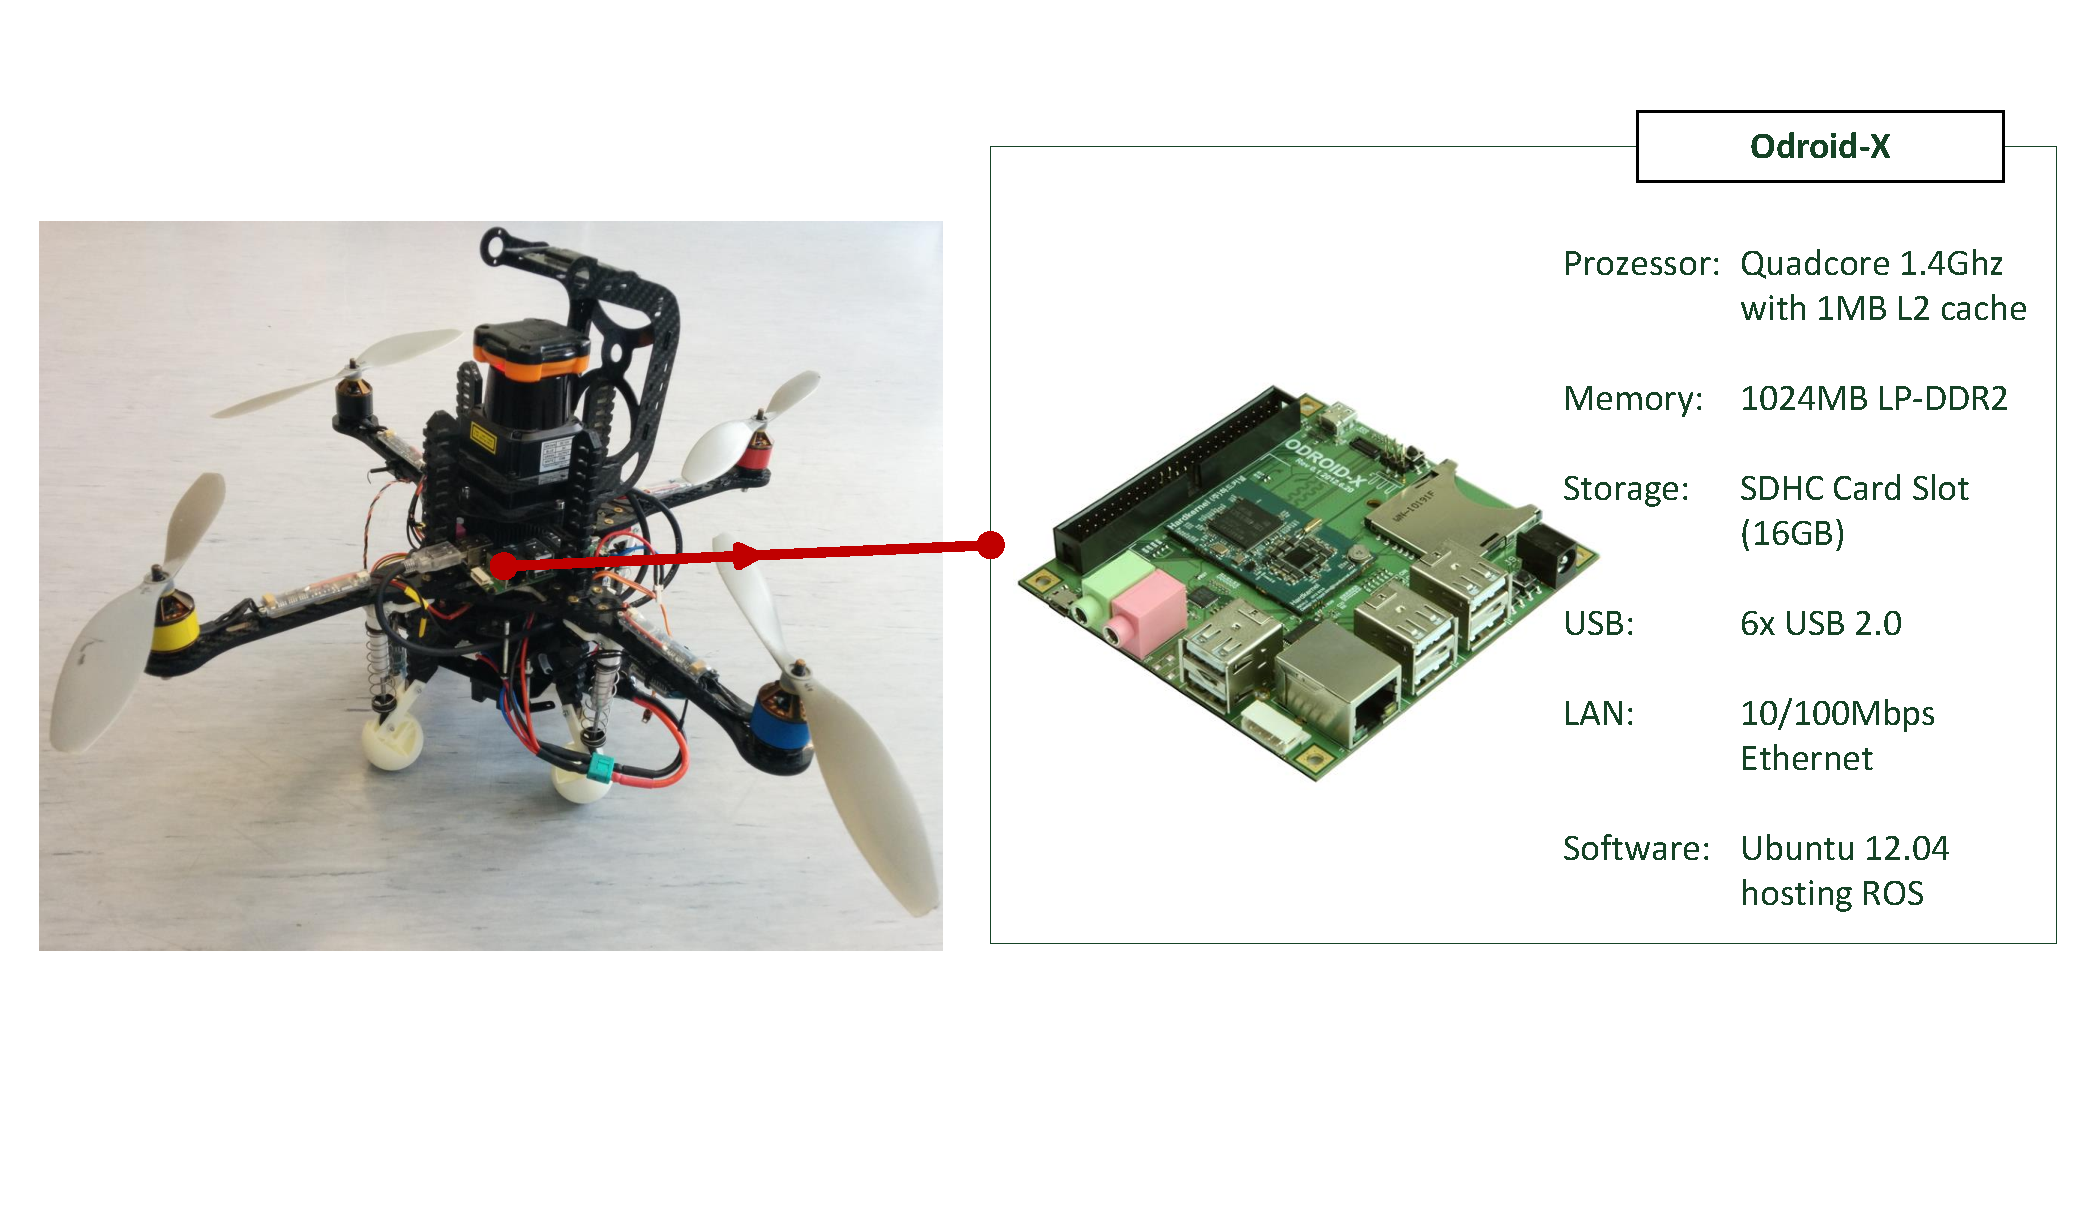
\includegraphics[width = 0.75\textwidth]{images/quad_odroid}
	\caption[Hardwareaufbau]{Hardwareaufbau des Quadrocopters...DIESE GRAFIK IST EIN PLATZHALTER GRAFIK NUR MIT NAMEN DER KOMPONENTEN}
	\label{fig:hardwareaufbau}
\end{figure}

\section{Kommunikationsstruktur}
\label{sec:Kommunikationsarchitekur}

Die Kommunikationsstruktur wird in Abbildung \ref{fig:Kommunikationsstruktur}
\begin{figure}
	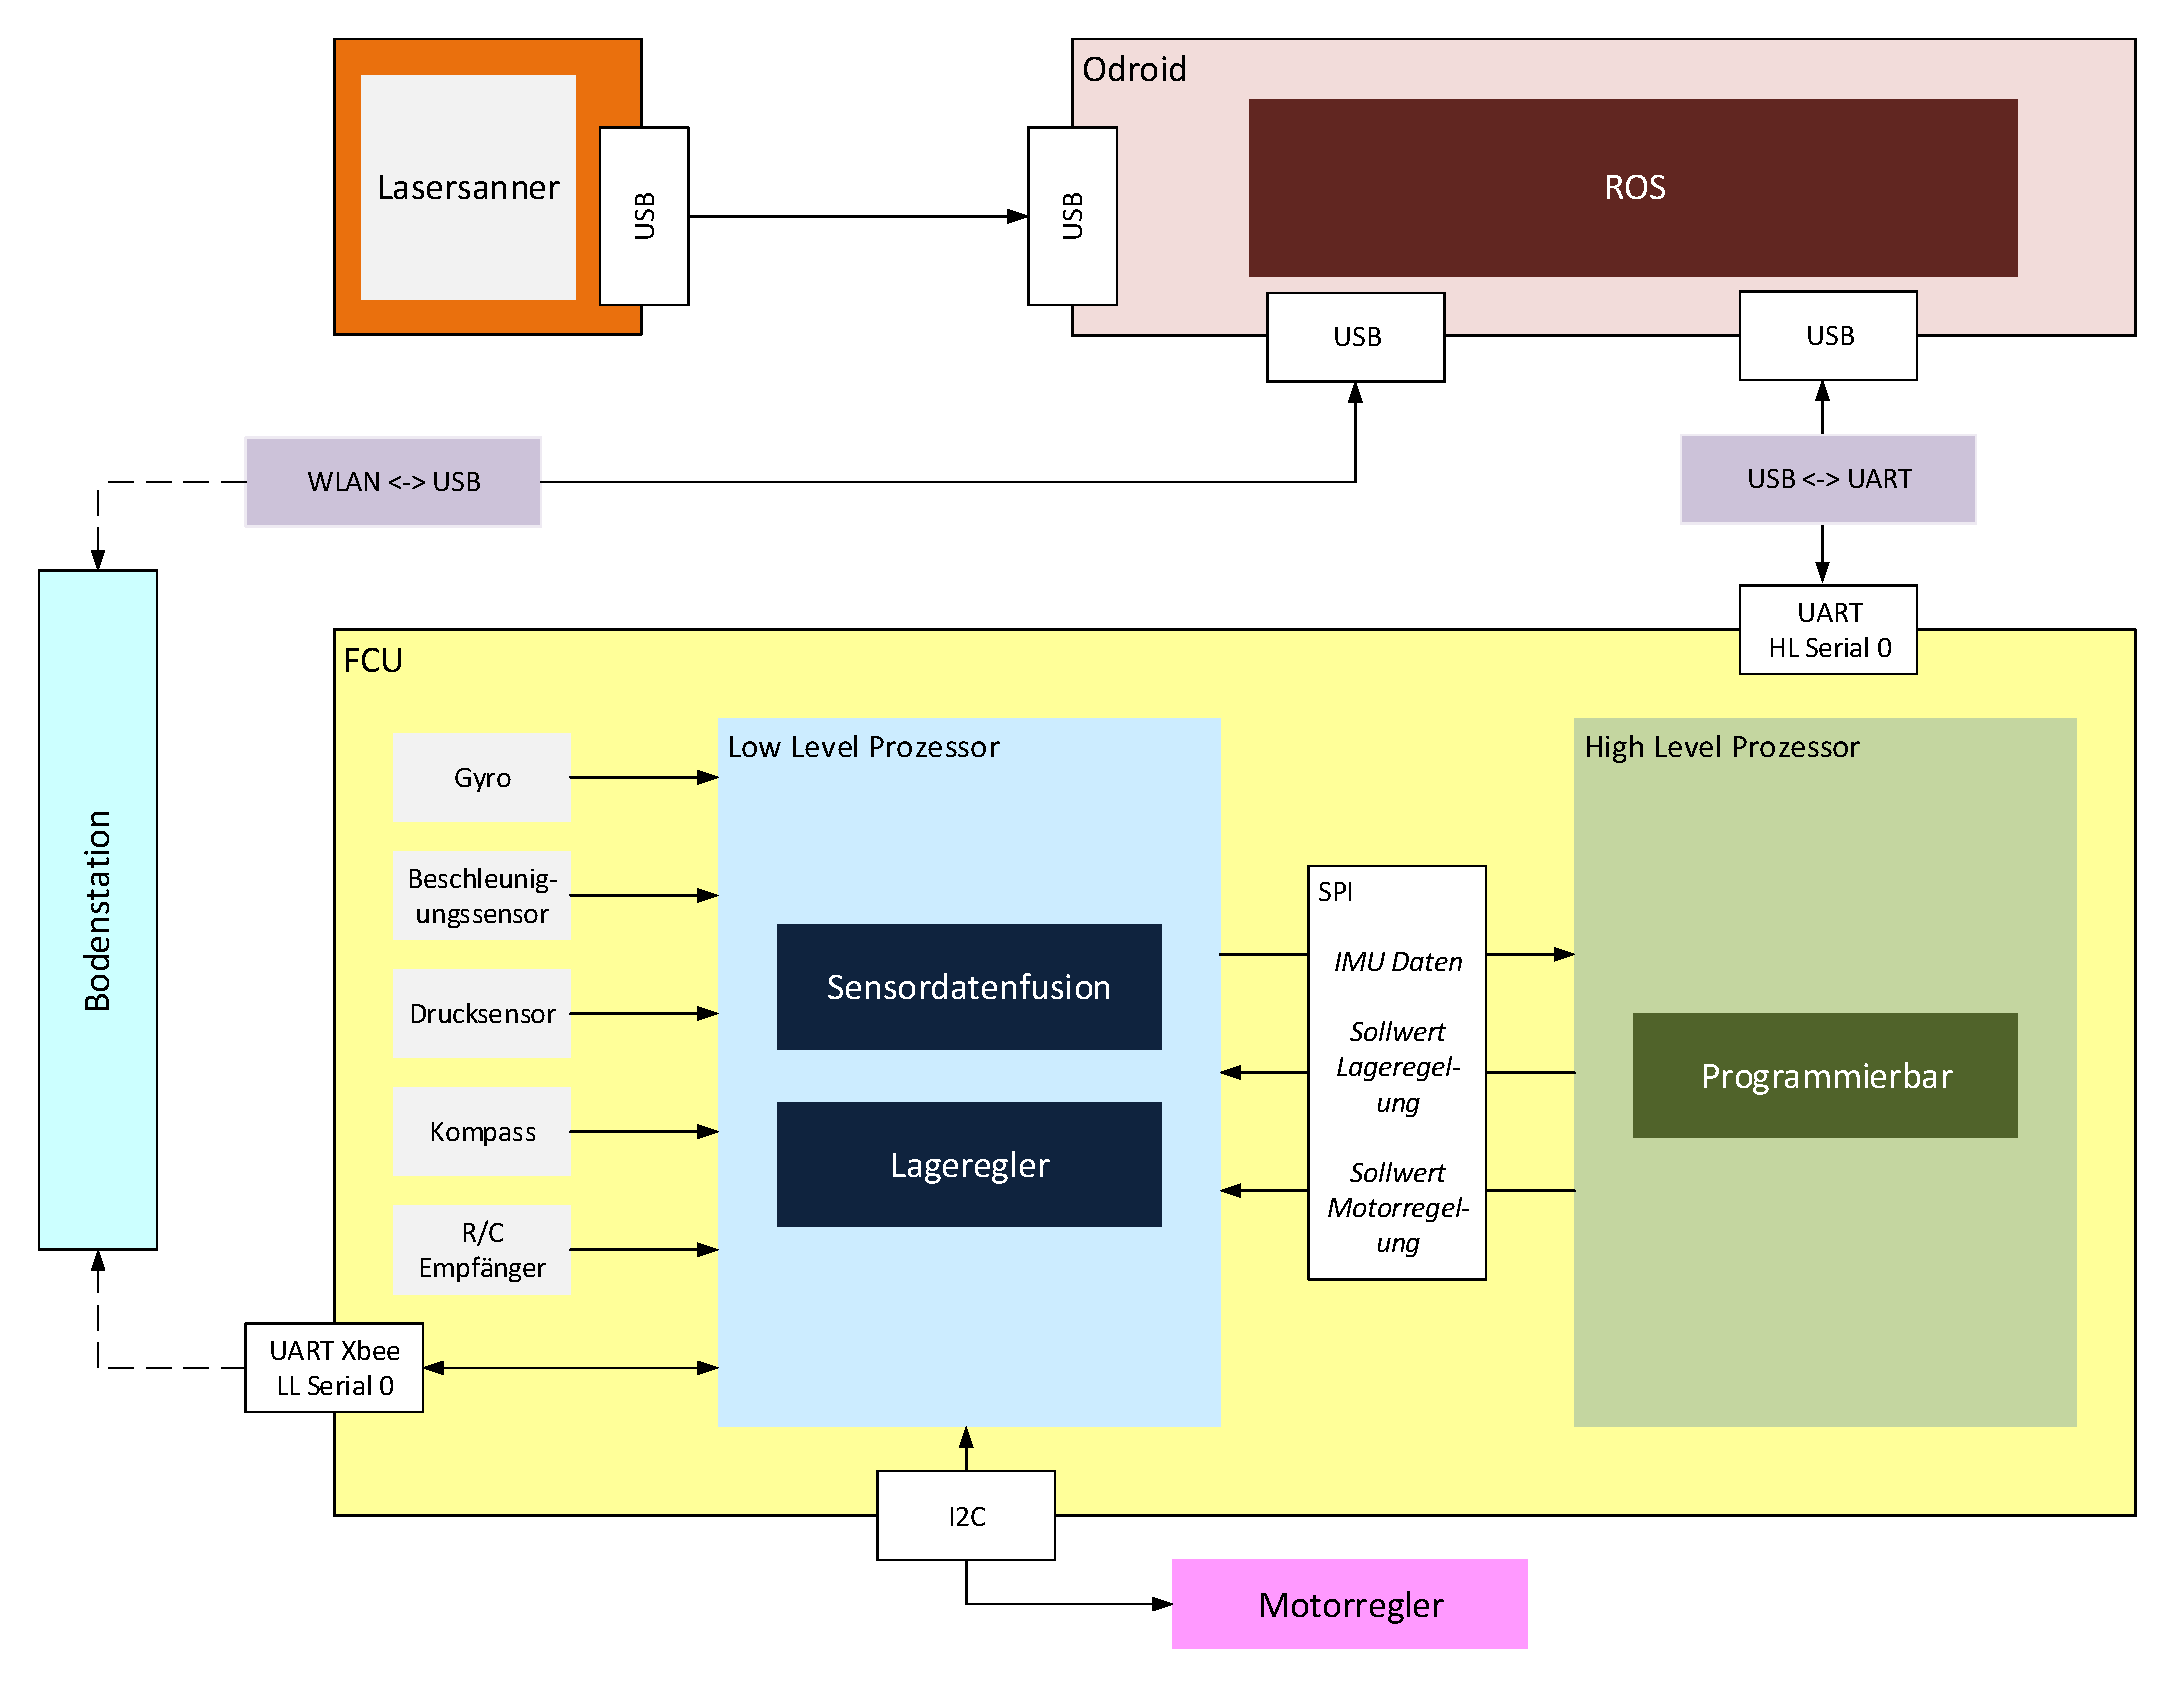
\includegraphics[width = \textwidth]{images/Kommunikationsarchitektur}
		\caption[Kommunikationsstruktur]{Kommunikationsstruktur des Quadrocopters  In Grafik fehlt das Modul zur H�henmessung Kompass auf deutsch}
		\label{fig:Kommunikationsstruktur}
\end{figure}
